
\chapter{Description de l'API de \PpFf}
\label{description.chap}

\gt{Pour \'eviter la confusion, tu dois utiliser les m\^emes termes
que dans l'API, m\^eme si ces termes sont en anglais. Mais tu les mets
dans la police courrier, avec texttt.}

\gt{Pas besoin de mettre API en \TT{API} --- c'est un acronyme, pas un
identificateur provenant du code source. Idem pour STL.}

\ic{J'ai enlev\'e l'API du titre et de la description de la figure}

\gt{Ce n'est pas ce que je voulais dire (de l'enlever).  C'\'etait
simplement la police de caract\`eres qui \'etait incorrecte!}

\begin{figure}[ht]
\centering
     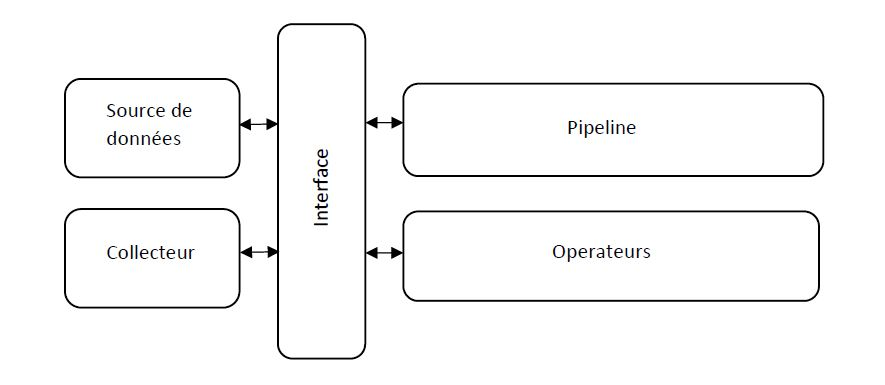
\includegraphics[width=1.0\textwidth]{Figures/ComponentsAPI.jpg}
      \caption{Les composants de l'API de \ppff.}
       \label{ComponentsAPI.fig}
\end{figure}


\gt{Pour ce premier diagramme de classes: il ne faudrait mettre que
les classes qui sont visibles aux utilisateurs, donc les <<concepts>>
qui sont utiles pour utiliser l'API et \^etre capable de s'en
servir. Les autres classes de plus bas niveau (en lien avec FastFlow
par exemple), pourront \^etre pr\'esent\'ees dans le prochain
chapitre.}

\ic{J'ai mis dans le diagramme seulement les classes qui sont visibles aux utilisateurs.}

Ce chapitre pr\'esente l'API de \ppff. Sa conception permet aux utilisateurs de tirer parti de la simplicit\'e d'utilisation tout en cachant la complexit\'e concernant les m\'ecanismes concurrents utilis\'es. La figure~\ref{ComponentsAPI.fig} pr\'esente une vue d'ensemble de l'architecture de \ppff. L'API est compos\'ee de quatre \'el\'ements principaux: l'Interface avec laquelle le d\'eveloppeur interagit, les \TT{Pipeline}s --- qui sont le coeur de l'API ---, les \TT{Stage}s et les \TT{Operator}s. Le r\^ole de chaque composant dans l'API est pr\'esent\'e dans la section suivante. La derni\`ere section  d\'ecrit plus en d\'etail les principales m\'ethodes de l'interface.

\gt{La macro \PpFf{} permet de g\'en\'erer la forme correcte, et
partout pareille. Une version sans majuscule, plus simple \`a
utiliser, produit la m\^eme chose.}

L'{API} de \PpFf{} est impl\'ement\'ee au-dessus de la biblioth\`eque \TT{FastFlow}, impl\'ementation qui sera d\'ecrite au prochain chapitre.

Le pr\'esent chapitre d\'ecrit le r\^ole de chaque composant de
\PpFf{}. La figure~\ref{ClassDiagramme.fig} pr\'esente une vue
d'ensemble des classes qui composent l'{API}.


%\gt{Note que de fa\c{c}on g\'en\'erale, lorsqu'on d\'ebute une section
%qui contient plusieurs sous-sections, il est pr\'ef\'erable d'avoir
%quelques lignes d'introduction, qui donnent une vue d'ensemble de ce
%qui suit. Pas toujours, mais ici, avec le diagramme de classes, \c{c}a
%ferait l'affaire.}
%
%\IC{Mon plan initial \'etait de d\'ecrire les composants dans le chapitre 2 (Description de l'API de \PpFf) et de pr\'esenter la partie technique dans le chapitre 3 (Impl\'ementation). Dans la premi\`ere partie du chapitre 2 j'ai choisi de d\'ecrire les composants principaux de l'API et dans la deuxi\`eme partie de ce chapitre de pr\'esenter quelques m\'ethodes avec des exemples. 
%Dans le chapitre 3 j'ai eu l'intention d'introduire un diagramme de classe UML en expliquant les classes qui compose l'API. } 
%
%\IC{Qu'est-ce que vous en pensez ? Est-ce que je dois introduire le diagramme dans le chapitre 2 ? Je ne suis pas sûr que je fasse la différence entre la description et implémentation de l’API.
%}


%\gt{La description est tout ce qu'un programmeur doit savoir/connaitre
%pour \underline{utiliser} ton API --- de l'ext\'erieur, comme une
%boite noire. L'impl\'ementation d\'ecrit les <<d\'etails>>
%n\'ecessaires pour comprendre \underline{comment fonctionne} l'API,
%par exemple, ce qu'un mainteneur devrait comprendre/connaitre s'il
%voulait modifier, corriger ou \'etendre ton API.}
%
%\gt{En lien avec le diagramme de classes, si l'utilisateur de l'API
%utilise ou manipule diff\'erents concepts et classes dans son
%programme, que ces concepts/classes sont utiles pour pouvoir utiliser
%correctement l'API --- avec la bonne syntaxe et la bonne s\'emantique
%--- alors ces concepts devraient \^etre d\'ecrits, par un diagramme de
%classes par exemple.}


\newpage
\KOMAoptions{paper=landscape,pagesize}
\recalctypearea

\begin{figure}[H]
\centering
     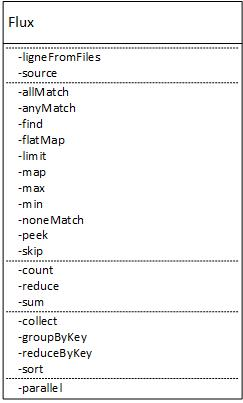
\includegraphics[width=\textwidth]{Figures/ClassDiagramme.jpg}
      \caption{Les classes qui composent l'{API}.}
       \label{ClassDiagramme.fig}
\end{figure}

\newpage
\KOMAoptions{paper=portrait,pagesize}
\recalctypearea



\section{Interface}

L'interface propos\'ee en \PpFf\ consiste en un ensemble de m\'ethodes qui permettent \`a l'utilisateur de manipuler des flux de donn\'ees de mani\`ere simple et efficace. L'interface suit d'assez pr\`es celle introduite pour les \emph{Streams} de Java~8. Le tableau~\ref{methodes_api.tab} d\'ecrit bri\`evement les m\'ethodes impl\'ement\'ees dans l'API.




%\gt{Dans un tabular, pour mettre du texte, on utilise p avec une
%largeur. Ceci \'evite de mettre des sauts de lignes explicites, ce qui
%n'est jamais une bonne id\'ee.}

%\ic{J'ai ajout\'e toutes les m\'ethodes d\'efinies dans l'interface de l'API dans ce tableau et j'ai \'et\'e oblig\'e d'utiliser le paquet longtable parce qu'elle s'\'etendait sur plusieurs pages. J'ai essay\'e de pr\'esenter la signature des m\'ethodes dans un format plus concis. Par exemple le paramètre std ::fonction a \'et\'e remplac\'e pour Func; j'ai enlev\'e les mots typename de chaque d\'eclaration de template; le param\`etre <typename ELEM, class ALLOC = std ::allocator<ELEM class TContainer >> a \'et\'e remplac\'e pour Container. De plus je n'ai pas pu r\'eutiliser la fonction qui redimensionne le tableau resizebox(textwidth). J'ai utilis\'e une police de caract\`ere plus petite (tiny) pour pouvoir encadrer le tableau dans la page.
%}
%
%\IC{J'ai reformul\'e la description pour le r\'esultat de la fonction flatMap}


%\begin{landscape}
\newpage
\KOMAoptions{paper=landscape,pagesize}
\recalctypearea


\begin{center}
\footnotesize
\begin{longtable}{|l|l|p{5cm}|}
\caption{Les m\'ethodes publiques de l'API de~\ppff.\label{methodes_api.tab}}\\
\hline
\textbf{M\'ethode} & \textbf{Type du r\'esultat} & \textbf{Description du r\'esultat}\\
\hline
\endfirsthead
\multicolumn{3}{c}%
{\tablename\ \thetable\ Méthodes publiques de l'API (\textit{suite})} \\
\hline
\textbf{M\'ethode} & \textbf{Type du r\'esultat} & \textbf{Description du r\'esultat}\\
\hline
\endhead
\hline \multicolumn{3}{r}{\textit{Suite page suivante}} \\
\endfoot
\hline
\endlastfoot
\hline
	\begin{tabular}{@{}l@{}}
	\tt template<T> \\
	\tt allMatch(Func<bool(T*)> predicate)
	\end{tabular} &
  	\TT{bool} &
    Retourne \TT{true} si tous les \'el\'ements
    du flux satisfont \TT{predicate}, sinon \TT{false}.
    \\
\hline
	\begin{tabular}{@{}l@{}}
	\tt template<T> \\
	\tt anyMatch(Func<bool(T*)> predicate)
	\end{tabular} &
  	\TT{bool} & 
    Retourne \TT{true} si au moins un  
    \'el\'ement du flux satisfait \TT{predicate}, sinon \TT{false}.
\\
\hline
	\begin{tabular}{@{}l@{}}
	\tt template<T, Container<T>{>}\\
	\tt collect()
	\end{tabular} &
  	\TT{Container<T>} &
    Retourne un conteneur
    STL avec tous les \'el\'ements du flux.
    \\
\hline
	\begin{tabular}{@{}l@{}}
	\tt count()\\
	\end{tabular} &
  	\TT{unsigned int} & 
    Retourne le nombre d'\'el\'ements
    du flux.
    \\
\hline
	\begin{tabular}{@{}l@{}}
	\tt template<In> \\
	\tt find(Func<bool(In*)> const\& predicate)
	\end{tabular} &
  	\TT{Pipe\&} &
    Retourne les
    \'el\'ements du flux qui satisfont \TT{predicate}.
    \\
\hline
	\begin{tabular}{@{}l@{}}
	\tt template<In, Out, Container> \\
	\tt flatMap(Func<Container*(In*)> const\& taskFunc)
	\end{tabular} &
  	\TT{Pipe\&} & 
    Applique la fonction fournie en argument
    \`a chaque \'el\'ement du flux et concat\`ene ces \'el\'ements lorsque plusieurs sont produits par la fonction.
    \\
\hline
	\begin{tabular}{@{}l@{}}
	\tt template<In, Out, Container=In> \\
	\tt flatMap()
	\end{tabular} &
  	\TT{Pipe\&} &
    Produit un flux avec les \'el\'ements du conteneur.  
    \\
\hline
	\begin{tabular}{@{}l@{}}
	\tt template<In, K=In, V=In, MapType> \\
	\tt groupByKey(Func<K*(In*)> fk, Func<V*(In*)> fv)
	\end{tabular} &
  	\TT{MapType} &
    Retourne un dictionnaire (\emph{map}) avec les \'el\'ements
    du flux regroupés par cl\'e.
   \\
\hline
%	\begin{tabular}{@{}l@{}}
%	\tt template<T, Container> \\
%	\tt intermediateCollect()
%	\end{tabular} &
%	\TT{Collection<T, Container>} &
%    Retourne une collection avec les
%    \'el\'ements du flux. 
%    \\ 
%\hline
	\begin{tabular}{@{}l@{}}
	\tt template<T> \\
	\tt limit(int n)
	\end{tabular} &
	\TT{Pipe\&} & 
    Retourne un flux compos\'e des \TT{n}~premiers \'el\'ements du flux d'entr\'ee.
    \\
\hline
	\begin{tabular}{@{}l@{}}
	\tt linesFromFile(string\& path)
	\end{tabular} &
	\TT{Pipe\&} & 
    Retourne un flux avec les lignes
    contenues dans le fichier indiqu\'e par \TT{path}.
    \\
\hline
	\begin{tabular}{@{}l@{}}
	\tt template<In, Out> \\
	\tt map(Func<Out*(In*)> const\& taskFunc)
	\end{tabular} &
	\TT{Pipe\&} & 
    Retourne un flux compos\'e de
    l'application de \TT{taskFunc}
    \`a chacun des
    \'el\'ements du flux.
    \\
\hline
	\begin{tabular}{@{}l@{}}
	\tt template<T> \\
	\tt max(Func<void(T*, T*)> compare)
	\end{tabular} &
	\TT{T} &
	Retourne l'\'el\'ement maximum du flux en fonction du comparateur.
    \\
\hline
	\begin{tabular}{@{}l@{}}
	\tt template<T> \\
	\tt min(Func<void(T*, T*)> compare)
	\end{tabular} &
	\TT{T} &
	Retourne l'\'el\'ement minimum du flux en fonction du comparateur.
    \\
\hline
	\begin{tabular}{@{}l@{}}
	\tt template<T> \\
	\tt noneMatch(Func<bool(T*)> predicate)
	\end{tabular} &
	\TT{bool} &
    Retourne \TT{true} si aucun des \'el\'ements
    du flux ne satisfait \TT{predicate},
    sinon \TT{false}.
    \\
\hline
	\begin{tabular}{@{}l@{}}
	\tt parallel(int workers = 1)
	\end{tabular} &
	\TT{Pipe\&} &
	Sp\'ecifie le nombre de travailleurs \`a utiliser pour traiter les \'el\'ements du flux.
    \\
\hline
	\begin{tabular}{@{}l@{}}
	\tt template<In> \\
	\tt peek(Func<void(In*)> const\& taskFunc)
	\end{tabular} &
	\TT{Pipe\&} &
	Applique la fonction \TT{taskFunc} \`a chaque \'el\'ement du flux et r\'e\'emet l'\'el\'ement (sans le modifier) sur le flux de sortie. Note: Utile pour le d\'ebogage.
    \\
\hline
	\begin{tabular}{@{}l@{}}
	\tt template<In, Out=In> \\
	\tt reduce(Reducer<In, Out> const\& reducer)
	\end{tabular} &
	\TT{Out} &
	Effectue une r\'eduction sur les \'el\'ements du flux. Voir la notion de \TT{reducer}, p.~\pageref{reducer.sect}.
    \\
\hline
	\begin{tabular}{@{}l@{}}
	\tt template<In, Out=In> \\
	\tt reduce(Out init, Func<Out(In, Out)> acc)
	\end{tabular} &
	\TT{Out} &
	Effectue une r\'eduction des \'el\'ements du flux, en utilisant \TT{init} comme valeur initiale et \TT{acc} comme fonction d'accumulation.
    \\
\hline
	\begin{tabular}{@{}l@{}}
	\tt template<In, K=In, V=In, MapType> \\
	\tt reduceByKey(Reducer<In, V> r, Func<K*(In*)> fk)
	\end{tabular} &
	\TT{MapType} &
    Effectue une r\'eduction sur les valeurs de chaque cl\'e à l'aide d'op\'erateur \TT{Reducer}. Voir la notion de \TT{Reducer}, p.~\pageref{reducer.sect}.
    \\
\hline
	\begin{tabular}{@{}l@{}}
	\tt template<T> \\
	\tt skip(int n)
	\end{tabular} &
	\TT{Pipe\&} &
    Retourne un flux compos\'e des \'el\'ements du flux d'entr\'ee, mais en omettant les \TT{n} premiers \'el\'ements.
    \\
\hline
	\begin{tabular}{@{}l@{}}
	\tt template<T> \\
	\tt sort(Func<bool(T, T)> const\& compare)
	\end{tabular} &
	\TT{Collection<T, Container>} &
	Effectue le tri des \'el\'ements du flux, selon l'ordre sp\'ecifi\'e par \TT{compare}. Note: Le premier \'el\'ement du flux de sortie n'est \'emis \emph{qu'apr\`es que la fin de flux ait \'et\'e rencontr\'ee}.
    \\
\hline
	\begin{tabular}{@{}l@{}}
	\tt template<T, Iterator> \\
	\tt source(Iterator  begin, Iterator end)
	\end{tabular} &
	\TT{Pipe\&} &
	Convertit un conteneur de type {STL} en flux.
    \\
\hline
	\begin{tabular}{@{}l@{}}
	\tt template<T> \\
	\tt sum()
	\end{tabular} &
	\TT{T} &
	Retourne la somme des \'el\'ements du flux.
    \\
\hline
\end{longtable}
\normalsize
\end{center}




%\end{landscape}
\newpage
\KOMAoptions{paper=portrait,pagesize}
\recalctypearea







%\begin{table}[h]
%\centering
%
%\resizebox{\textwidth}{!}{%
%
%\begin{tabular}{|l|l|p{8cm}|}
%\hline
%\textbf{M\'ethode} & \textbf{Type du r\'esultat} & \textbf{Description du r\'esultat}\\
%\hline
%	\begin{tabular}{@{}l@{}}
%	\tt template<T> \\
%	\tt allMatch(Func<bool(T*)> predicate)
%	\end{tabular} &
%  	\TT{bool} &
%    Retourne \TT{true} si tous les \'el\'ements
%    du flux correspondent au pr\'edicat
%    fourni, sinon \texttt{false}.
%    \\
%\hline
%	\begin{tabular}{@{}l@{}}
%	\tt template<T> \\
%	\tt anyMatch(Func<bool(T*)> predicate)
%	\end{tabular} &
%  	\texttt{bool} & 
%    Retourne \texttt{true} si au moins un  
%    \'el\'ement du flux correspondent
%    au pr\'edicat fourni, sinon \texttt{false}.
%\\
%\hline
%	\begin{tabular}{@{}l@{}}
%	\tt template<T, Container<T>>\\
%	\tt collect()
%	\end{tabular} &
%  	\texttt{Container<T>} &
%    Retourne un conteneur de type
%    STL contenant les \'el\'ements du flux.
%    \\
%\hline
%	\begin{tabular}{@{}l@{}}
%	\tt count()\\
%	\end{tabular} &
%  	\texttt{unsigned int} & 
%    Retourne le nombre d'\'el\'ements
%    dans ce flux.
%    \\
%\hline
%	\begin{tabular}{@{}l@{}}
%	\tt template<In> \\
%	\tt find(Func<bool(In*)> const\& taskFunc)
%	\end{tabular} &
%  	\texttt{Pipe\&} &
%    Retourne tous les
%    \'el\'ements du flux qui satisfont la 
%    fournie en argument.
%    \\
%\hline
%	\begin{tabular}{@{}l@{}}
%	\tt template<In, Out, Container> \\
%	\tt flatMap(Func<Container*(In*)> const\& taskFunc)
%	\end{tabular} &
%  	\texttt{Pipe\&} & 
%    Applique la fonction fournie en argument
%    \`a chaque \'el\'ement du flux.
%    \\
%\hline
%	\begin{tabular}{@{}l@{}}
%	\tt template<In, Out, Container=In> \\
%	\tt flatMap()
%	\end{tabular} &
%  	\texttt{Pipe\&} &
%    \GT{Reformuler: je ne comprends pas la diff\'erence avec le pr\'ec\'edent}    
%    \\
%\hline
%	\begin{tabular}{@{}l@{}}
%	\tt template<In, K=In, V=In, MapType> \\
%	\tt groupByKey(Func<K*(In*)> fk, Func<V*(In*)> fv)
%	\end{tabular} &
%  	\texttt{MapType} &
%    Retourne un dictionnaire (\emph{map}) avec les \'el\'ements
%    du flux regroupés par cl\'e.
%   \\
%\hline
%	\begin{tabular}{@{}l@{}}
%	\tt template<T, Container> \\
%	\tt intermediateCollect()
%	\end{tabular} &
%	\texttt{Collection<T, Container>} &
%    Retourne une collection avec les
%    \'el\'ements du flux.
%    \\ 
%\hline
%	\begin{tabular}{@{}l@{}}
%	\tt template<T> \\
%	\tt limit (int n)
%	\end{tabular} &
%	Pipe\& & 
%    Renvoie dans le flux seulement
%    les n premiers \'el\'ements de
%    ce flux.
%    \\
%\hline
%	\begin{tabular}{@{}l@{}}
%	\tt linesFromFile(string\& path)
%	\end{tabular} &
%	Pipe\& & 
%    Renvoie dans le flux les lignes
%    contenues dans un fichier.
%    \\
%\hline
%	\begin{tabular}{@{}l@{}}
%	\tt template<In, Out> \\
%	\tt map(Func<Out*(In*)> const\& taskFunc)
%	\end{tabular} &
%	Pipe\& &
%    Renvoie dans le flux les
%    r\'esultats constitu\'es de 
%    l'application d'une fonction 
%    fournie en param\`etre aux 
%    \'el\'ements du flux.
%    \\
%\hline
%	\begin{tabular}{@{}l@{}}
%	\tt template<T> \\
%	\tt max(Func<void(T*, T*)> compare)
%	\end{tabular} &
%	\texttt{T} &
%	Retourne l'\'el\'ement maximum du flux en fonction du comparateur fourni en param\`etre.
%    \\
%\hline
%	\begin{tabular}{@{}l@{}}
%	\tt template<T> \\
%	\tt min(Func<void(T*, T*)> compare)
%	\end{tabular} &
%	\texttt{T} &
%	Retourne l'\'el\'ement minimum du flux en fonction du comparateur fourni en param\`etre.
%    \\
%\hline
%	\begin{tabular}{@{}l@{}}
%	\tt template<T> \\
%	\tt noneMatch(Func<bool(T*)> predicate)
%	\end{tabular} &
%	\texttt{bool} &
%	Retourne l'\'el\'ement minimum du flux en fonction du comparateur fourni en param\`etre.
%    \\
%\hline
%	\begin{tabular}{@{}l@{}}
%	\tt parallel(int workers = 1)
%	\end{tabular} &
%	Pipe\& &
%	D\'efinis le nombre de travailleurs fourni en param\`etre.
%    \\
%\hline
%	\begin{tabular}{@{}l@{}}
%	\tt template<In> \\
%	\tt peek(Func<void(In*)> const\& taskFunc)
%	\end{tabular} &
%	Pipe\& &
%	M\'ethode utilis\'ee pour d\'ebogage. Applique une fonction sur les \'el\'ements du flux sans modifier leur valeur.
%    \\
%\hline
%	\begin{tabular}{@{}l@{}}
%	\tt template<In, Out=In> \\
%	\tt reduce(Reducer<In, Out> const\& reducer)
%	\end{tabular} &
%	\texttt{Out} &
%	reduce description.
%    \\
%\hline
%	\begin{tabular}{@{}l@{}}
%	\tt template<In, Out=In> \\
%	\tt reduce(Out init, Func<Out(In, Out)> acc)
%	\end{tabular} &
%	\texttt{Out} &
%	reduce description.
%    \\
%\hline
%	\begin{tabular}{@{}l@{}}
%	\tt template<In, K=In, V=In, MapType> \\
%	\tt reduceByKey(Reducer<In, V> r, Func<K*(In*)> fk)
%	\end{tabular} &
%	\texttt{MapType} &
%	reduceByKey description.
%    \\
%\hline
%	\begin{tabular}{@{}l@{}}
%	\tt template<T> \\
%	\tt skip(int n)
%	\end{tabular} &
%	Pipe\& &
%	skip description.
%    \\
%\hline
%	\begin{tabular}{@{}l@{}}
%	\tt template<T> \\
%	\tt sort(Func<bool(T, T)> const\& compare)
%	\end{tabular} &
%	\texttt{Collection<T, Container>} &
%	sort description.
%    \\
%\hline
%	\begin{tabular}{@{}l@{}}
%	\tt template<T, Iterator> \\
%	\tt source(Iterator  begin, Iterator end)
%	\end{tabular} &
%	Pipe\& &
%	source description.
%    \\
%\hline
%	\begin{tabular}{@{}l@{}}
%	\tt template<T> \\
%	\tt sum()
%	\end{tabular} &
%	\texttt{T} &
%	sum description.
%    \\
%\hline
%
%
%\end{tabular}
%}
%\caption{Les m\'ethodes expos\'ees aux utilisateurs par l'API de \ppff.}
%\label{methodes_api.tab}
%\end{table}




Comme on peut le voir dans le tableau~\ref{methodes_api.tab}, la d\'eclaration des m\'ethodes utilise la programmation g\'en\'erique de C++, c'est-\`a-dire les \emph{templates}. Cela permet aux utilisateurs d'avoir une interface g\'en\'erique unique, de sorte qu'une m\'ethode peut \^etre r\'eutilis\'ee pour n'importe quel type de donn\'ees.


Un autre point cl\'e dans cette interface est son expressivit\'e. M\^eme avant sa conception d\'etaill\'ee, nous nous \'etions donn\'es comme objectif de fournir un syst\`eme suffisamment intuitif et expressif pour le traitement de flux de donn\'ees. 

\gt{Lorsque dans le texte tu indiques des identificateurs qui viennent du code --- find, collect, etc. --- alors il faut les mettre en police tt, donc \TT{find}, \TT{collect}, etc.}


\gt{Comme indiqu\'e dans le chapitre pr\'ec\'edent, oublie ce que
j'avais \'ecrit concernant l'environnement Listing, car cela ne
produit pas le bon num\'ero, tel qu'officiellement requis par le guide
UQAM (2.1, 2.2, etc.).  Il faut plut\^ot utiliser les diverses options
associ\'ees directement \`a lstlisting. Pour rappel, voir le chapitre
pr\'ec\'edent ainsi que l'exemple de Reducer un peu plus bas.}


\ic{J'ai v\'erifi\'e le terme listing dans tout le document. Vous les avez remplac\'es par tout. }


%
% Tu as deja ce listing plus bas!?
% \begin{lstlisting}[
% label={reducer.c++},
% language=c++,
% caption={La signature d'un objet \TT{Reducer}.},
% frame=single,
% float]
%  template<typename In, typename Out>
%  class Reducer {
%        Reducer(Out init, 
%                Func<Out(Out, In)> const& accumulator,
%                Func<Out(Out, Out)> const& combiner)

%        Reducer(Func<Out(Out, In)> const& accumulator,
%                Func<Out(Out, Out)> const& combiner)

%        Reducer(Out init, 
%                Func<Out(Out, In)> const& accumulator)
%  }
% \end{lstlisting}


\begin{lstlisting}[
label={expressivite_api.c++},
language=c++,
caption={Un exemple illustrant les principaux \'el\'ements de l'API de \ppff.},
frame=single,
float]
// Definition (omise) d'un vecteur d'objets Employee.
std::vector<Employee> sourceEmployees;
...

std::vector<Employee> result = 
   Pipe()
   .source<Employee>(sourceEmployees.begin(), sourceEmployees.end())
   .find<Employee>([](Employee *e) { return e->salary > 35000; })
   .collect<Employee, std::vector>();
\end{lstlisting}




Le listing~\ref{expressivite_api.c++} pr\'esente un extrait de code C++ qui donne un premier aper\c{c}u de l'expressivit\'e de l'interface --- d'autres exemples seront pr\'esent\'es plus loin. Dans cet exemple, on s\'electionne les employ\'es qui ont un salaire plus grand que 35~K\$. Les employ\'es sont initialement dans un conteneur STL et sont filtr\'es en chainant trois op\'erations : $i)$ \TT{source} qui permet d'envoyer dans le flux des objets de type~\TT{Employe}; $ii$) \TT{find} qui s\'electionne les employ\'es selon la condition fournie en param\`etre (une lambda-expression); $iii)$ \TT{collect} qui met les employ\'es s\'electionn\'es dans un conteneur STL. Ici, les employ\'es s\'electionn\'es sont mis dans un conteneur de type \TT{std::vector} --- le type de conteneur est donn\'e par le type fourni en argument (g\'en\'erique) de la m\'ethode \TT{collect}.




\section{Op\'erateurs}

Les op\'erateurs (classe \TT{Operator}) sont la base de notre syst\`eme. L'API fournit un ensemble d'op\'erateurs qui facilitent la t\^ache de l'utilisateur. Les op\'erateurs sont structur\'es en deux cat\'egories : les op\'erateurs sans \'etat et les op\'erateurs avec \'etat.

Les \emph{op\'erateurs sans \'etat} sont ceux qui ne disposent pas d'informations sur l'it\'eration en cours et ne transmettent pas les informations interm\'ediaires des \'etapes de traitement pr\'ec\'edentes. Si on prend comme exemple le filtre repr\'esent\'e par la m\'ethode \TT{find} du tableau~\ref{methodes_api.tab}, il traite le flux de donn\'ees \'el\'ement par \'el\'ement. 
%
Lorsque la fonction (lambda-expression) fournie en argument \`a la m\'ethode \TT{find} ne satisfait pas la condition lorsqu'appliqu\'ee \`a un \'el\'ement du flux, le filtre ne retourne rien. 

Les \emph{op\'erateurs avec \'etat} sont ceux qui maintiennent une structure de donn\'ees interne, qui repr\'esente l'\'etat. Cette structure repr\'esente ou synth\'etise l'historique des \'el\'ements pass\'es au flux et affecte la logique de traitement dans les calculs ult\'erieurs. Par exemple, l'op\'erateur \TT{Sum} calcule la somme des \'el\'ements du flux. Son \'etat contient la valeur de la somme de tous les \'el\'ements qui pr\'ec\'edent celui en cours de traitement. 

\subsection*{Op\'erateurs de r\'eduction}

\label{reducer.sect}

\begin{lstlisting}[
label={reducer.c++},
gobble=1,
language=c++,
caption={La signature d'un objet \TT{Reducer}.},
frame=single,
float]
 template<typename In, typename Out>
 class Reducer {
       Reducer(Out init, 
               Func<Out(Out, In)> const& accumulator,
               Func<Out(Out, Out)> const& combiner)

       Reducer(Func<Out(Out, In)> const& accumulator,
               Func<Out(Out, Out)> const& combiner)

       Reducer(Out init, 
               Func<Out(Out, In)> const& accumulator)

       Reducer(Func<Out(Out, In)> const& accumulator)
 }
\end{lstlisting}



\gt{Une règle utile à savoir pour \LaTeX: lorsqu'on met un élément
flottant (avec caption/label, e.g., figure, table, pseudocode,
listing), il est préférable de mettre cet élément \underline{avant} la
première référence (et non pas après).  La position du flottant par
rapport au texte qui y réfère est alors meilleure.}

L'op\'erateur de classe \TT{Reducer} est utilis\'e pour r\'eduire les \'el\'ements du flux \`a une valeur unique. Le listing~\ref{reducer.c++} présente la spécification  de la classe \TT{Reducer} avec les signatures des diverses fonctions associées. 


\begin{lstlisting}[
label={sumElementsCollectionWithReducer},
language=c++,
gobble=4,
caption={[Exemple d'utilisation de l'opérateur \TT{Reducer}.]Exemple
d'utilisation de l'opérateur \TT{Reducer}~: ici, les \'el\'ements
d'une collection sont simplement additionn\'es entre eux, avec
l'op\'erateur \TT{std::plus<int>\{\}}.},
frame=single,
float]
    int n = 100;
    std::vector<int> elems(n);
    for (unsigned int i = 0; i < elems.size(); i++) {
        elems[i] = i;
    };

    Reducer<int, int> reducer(std::plus<int>{});

    int currentResult =
        Pipe()
        .source<int>(elems.begin(), elems.end())
        .reduce<int, int>(reducer);

	std::cout << "Result: " << currentResult;	// == 4950   
\end{lstlisting}


\GT{J'ai chang\'e la description ci-bas. Ce n'\'etait pas vrai de
dire, il me semble, que la valeur initiale \'etait la valeur par
d\'efaut du type, car ce n'est pas cela que fait le code et, de toute
fa\c{c}on, tu ne peux pas connaitre cette valeur, non?}

La forme la plus g\'en\'erale d'un \TT{Reducer} est celle construite avec trois \'el\'ements: une valeur initiale, une fonction \TT{accumulator} et une fonction \TT{combiner}. La valeur initiale et la fonction \TT{combiner} sont optionnelles gr\^ace \`a la surcharge du constructeur. Lorsque ces arguments sont omis, la valeur initiale utilis\'ee est le premier \'el\'ement re\c{c}u et la fonction \TT{combiner} est simplement la fonction \TT{accumulator}. Par exemple, le listing~\ref{sumElementsCollectionWithReducer} montre un exemple d'utilisation de l'op\'erateur \TT{Reducer} avec un seul argument~: la valeur initiale n'est pas sp\'ecifi\'ee --- donc la collection \`a traiter doit contenir au moins un \'el\'ement --- et la fonction \TT{combiner}, si n\'ecessaire (voir plus bas) sera simplement la fonction \TT{accumulator}, i.e., l'addition \TT{std::plus<int>\{\}}.


\begin{lstlisting}[
label={sumElementsCollectionWithReducerParallel},
gobble=4,
language=c++,
caption={[Exemple d'utilisation de l'opérateur \TT{Reducer}, ex\'ecut\'e en
parall\`ele et avec une valeur initiale.]Exemple
d'utilisation de l'opérateur \TT{Reducer}, ex\'ecut\'e en parall\`ele et avec une
valeur initiale non nulle sp\'ecifi\'ee explicitement.},
frame=single,
float]
    int n = 100;
    std::vector<int> elems(n);
    for (unsigned int i = 0; i < elems.size(); i++) {
        elems[i] = i;
    };

    // Avec valeur initiale explicite... pour illustrer l'effet!
    Reducer<int, int> reducer(3, 
                              std::plus<int>{}, 
                              std::plus<int>{});

	int currentResult =
		Pipe()
		.source<int>(elems.begin(), elems.end())
		.parallel(2)
		.reduce<int, int>(reducer); 
	
	std::cout << "Result: " << currentResult;	// == 4953
\end{lstlisting}




Le troisi\`eme param\`etre de l'op\'erateur \TT{Reducer}, la fonction \TT{combiner}, est utilis\'e lorsque le flux est trait\'e en parall\`ele, par plusieurs \emph{threads}. Dans un tel cas, le flux est divis\'e en sous-flux --- i.e., chaque \emph{thread} traite un sous-ensembles des éléments --- qui sont r\'eduits en parall\`ele avec la fonction \TT{accumulator}. Les r\'esultats partiels produits par les divers \emph{threads} sont ensuite combin\'es, dans le \emph{thread} principal, avec la fonction \TT{combiner}. Le listing~\ref{sumElementsCollectionWithReducerParallel} montre un exemple d'utilisation de l'op\'erateur \TT{Reducer} mais ex\'ecut\'e en parall\`ele. Dans cet exemple, \`a des fins d'illustration, une valeur initiale est sp\'ecifi\'ee, \'egale \`a \TT3 et, alors que les fonctions \TT{combiner} et \TT{accumulator} sont toutes deux indiqu\'ees comme \'etant la fonction d'addition \TT{std::plus<int>\{\}}. 


\gt{R\'esultat incorrect indiqu\'e je crois: 4953 => 5053!?}

\ic{J’ai pris l’exemple des tests unitaires. La formule de calcul pour
le résultat attendu est~:  expectedResult = n * (n - 1) / 2;}


\newpage

\subsection*{Description formelle d'un \TT{Reducer}}

Soit les \'el\'ements suivants~: 
\begin{itemize}
\item $In$ et $Out$ des types de donn\'ees;

\item $S = [s_0, s_1, \ldots, s_k]$, un flux de donn\'ees, o\`u $s_i
\in In~(i=0, \ldots, k)$;

\item Soit $v_0\in Out$;

\item Soit $acc: Out\times In \rightarrow Out$;

\item Soit $comb: Out\times Out \rightarrow Out$;

\end{itemize}

Notons par~:
\begin{itemize}
\item   \TT{Reducer($acc$)} un objet \TT{Reducer} avec l'attribut $acc$~; 
\item   \TT{Reducer($v_0, acc$)} un objet \TT{Reducer} avec les attributs $v_0$ et $acc$.
\item   \TT{Reducer($v_0, acc, comb$)} un objet \TT{Reducer} avec les
attributs $v_0$, $acc$ et $comb$.
\end{itemize}

\bigskip

Pour les deux premiers types de \TT{Reducer}, on peut alors
repr\'esenter un appel \`a \TT{reduce} de fa\c{c}on graphiquement
comme illustr\'e dans la figure~\ref{reduce.fig}.%
%
\footnote{Plus formellement~:
%
\begin{eqnarray*}
S\TT{.reduce}(\TT{Reducer}(acc)) 
  &=& fold\ acc\ s_0\ [s_1, \ldots, s_k]
\\
S\TT{.reduce}(\TT{Reducer}(v_0, acc)) 
  &=& fold\ acc\ v_0\ [s_0, s_1, \ldots, s_k]
\\
\\
fold\ acc\ a\ [~]  
  &=& a
\\
fold\ acc\ a\ [s_0, s_1, \ldots, s_k] 
  &=& fold\ acc\ (acc\ a\ s_0)\ [s_1, \ldots, s_k]
\\
  &=& acc (\ldots (acc\ (acc\ a\ s_0)\ s_1) \ldots) s_k)
\end{eqnarray*}
}
 
\begin{figure}
\begin{minipage}{.05\linewidth}
\ \ 
\end{minipage}
%
\begin{minipage}{.4\linewidth}
\begin{alltt}
\(S\TT{.reduce}(\TT{Reducer}(v\sb0, acc)) =\)
         \(acc\)
         \(\slash\) \(\backslash\)
       \(acc\)  \(s\sb{k}\)
        \(\slash\) \(\backslash\)
       \vdots
      \(\slash\) \(\backslash\)
    \(acc\)  \(s\sb1\)
    \(\slash\) \(\backslash\)
  \(v\sb0\)   \(s\sb0\)
\end{alltt}
\end{minipage}
%
\begin{minipage}{.1\linewidth}
\ \ 
\end{minipage}
%
\begin{minipage}{.4\linewidth}
\begin{alltt}
\(S\TT{.reduce}(\TT{Reducer}(acc)) =\)
         \(acc\)
         \(\slash\) \(\backslash\)
       \(acc\)  \(s\sb{k}\)
        \(\slash\) \(\backslash\)
       \vdots
      \(\slash\) \(\backslash\)
    \(acc\)  \(s\sb2\)
    \(\slash\) \(\backslash\)
  \(s\sb0\)   \(s\sb1\)
\end{alltt}
\end{minipage}
\caption[Repr\'esentation graphique d'un appel \`a
\TT{reduce}.]{Repr\'esentation graphique d'un appel \`a
\TT{reduce}. Chaque n\oe{}ud interm\'ediaire, not\'e avec $acc$,
repr\'esente un appel \`a la fonction $acc$ avec deux arguments.}
\label{reduce.fig}
\end{figure}

\GT{Peut-\^etre serait-il pr\'ef\'erable d'avoir un <<vrai>>
graphique, plut\^ot que du texte comme dans le alltt ci-haut?}


\GT{Donnez ensuite quelques explications concernant un appel
\TT{S.reduce(Reducer($v_0, acc, comb$))}~: Les \'el\'ements de $S$
sont r\'epartis entre divers \emph{threads}, accumul\'es comme dans la
figure pour produire un r\'esultat interm\'ediaire par \emph{threads},
puis ces r\'esultats interm\'ediaires sont $comb$in\'es avec la
fonction $comb$.}
\newpage





\section{Pipeline}


\begin{figure}[ht]
\centering
     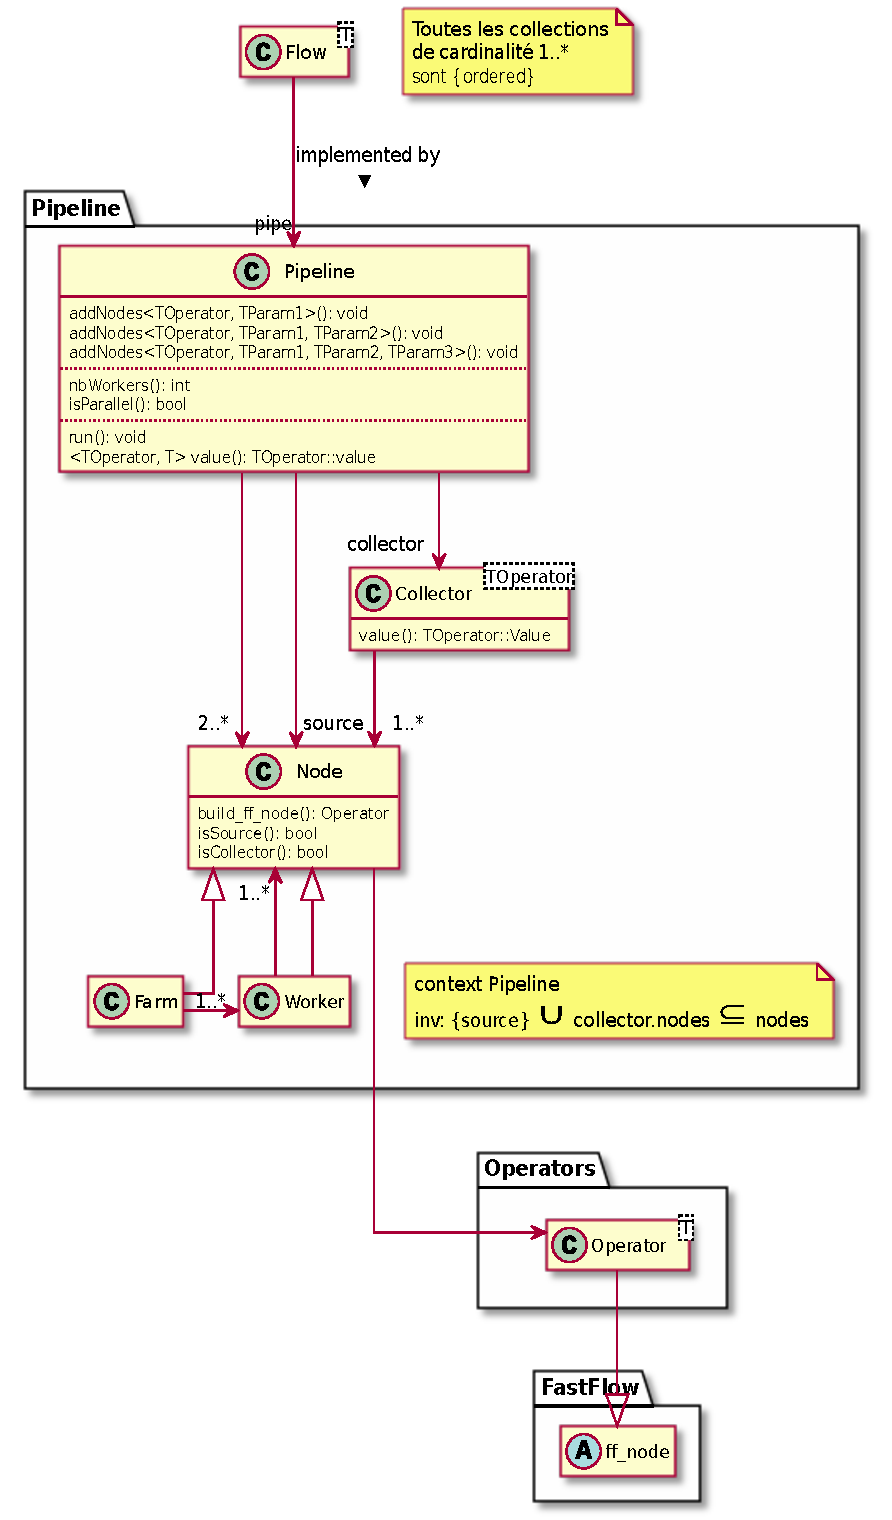
\includegraphics[width=1.0\textwidth]{Figures/Pipeline.jpg}
      \caption[Repr\'esentation graphique d'un pipeline.]{Une repr\'esentation graphique d'un pipeline.}
       \label{Pipeline.fig}
\end{figure}

Le \TT{Pipeline} est le composant principal de notre {API}. Un \TT{Pipeline} est une cha\^{\i}ne de traitement compos\'ee d'un ou plusieurs \TT{Operator}s regroup\'es dans des \TT{Stages}. La figure~\ref{Pipeline.fig} montre une vue d\'etaill\'ee d'un \TT{Pipeline} en action. Une \'etape de la cha\^{\i}ne de traitement de ce mod\`ele traite les donn\'ees produites par l'\'etape pr\'ec\'edente dans le flux et fournit les r\'esultats \`a l'étape suivante dans le flux. 

%Un pipeline \TT{P} avec $n$ \'etapes peut \^etre d\'efini comme suit:
%
%\[
%	\TT{P} = O_1 +  \ldots + O_k + \ldots + O_n
%\]
%
%Dans l'expression ci-dessus, $O_k$ d\'enote le $k^e$ op\'erateur dans le pipeline~\TT{P}.

\gt{Il faut clarifier la partie ci-haut. On ne comprends pas pourquoi
$P = O_1 + \ldots + O_n$ --- pourquoi <<+>>? Pourquoi ne pas utiliser
le symbole de pipe comme en Unix, i.e., <<$\vert$>>?  Ce serait plus
naturel peut-\^etre?  (Parce que dans plusieurs notations formelles,
<<+>> est utilis\'e pour repr\'esenter un {\bf choix}, et non une
s\'equence cons\'ecutive d'items.)}

\gt{En outre, on ne comprend pas le lien entre cette \'equation et la
figure.  Ce serait pr\'ef\'erable qu'on puisse comprendre quel est
exactement ce qui est repr\'esent\'e par la figure: il y a un premier
pipeline s\'equentiel, form\'e de 3 op\'erateurs, un autre parall\`ele
(form\'e de 4 op\'erateurs), puis un autre (de 2 op\'erateurs).
Sinon, on cherche \`a comprendre \`a quoi la figure correspond, quel
est le lien avrc l'\'equation. Parce qu'en ce moment, il me semble que
l'\'equation n'est pas utile --- elle le serait si elle \'etait
ensuite utilis\'ee plus loin, ailleurs, pour expliquer/repr\'esenter
autre chose, ce qui n'est pas le cas.}

\ic{J'ai enlev\'e l'expression formelle. La figure a \'et\'e ajout\'ee ult\'erieurement. Je n'ai pas pens\'e \`a un lien entre l'\'equation et la figure.}

L'utilisation de \TT{Pipeline} introduit une couche d'abstraction sur une cha\^{\i}ne complexe d'op\'erateurs. De plus, un \TT{Pipeline} n'expose à l'ext\'erieur que ses entr\'ees et ses sorties. Une telle conception modulaire permet une flexibilit\'e au syst\`eme tout en simplifiant la mise en œuvre. Par exemple, le parall\'elisme de donn\'ees
pourrait \^etre facilement r\'ealis\'e en ayant plusieurs \TT{Pipeline}s identiques connect\'es \`a la m\^eme entr\'ee et sortie. La figure~\ref{Pipeline.fig} illustre ce m\'ecanisme~: le parall\'elisme de donn\'ee est r\'ealis\'e en connectant plusieurs copies du m\^eme pipeline en parall\`ele. Ainsi, dans cette figure, l'entr\'ee pour les pipelines parall\`eles (compos\'es de quatre op\'erateurs) est la sortie du premier pipeline (s\'equentiel, compos\'e de trois op\'erateurs) et la sortie des pipelines parall\`eles est l'entr\'ee du pipeline qui suit (lui aussi s\'equentiel, compos\'e de deux op\'erateurs).


\section{Travailler avec des flux}

Cette section pr\'esente de fa\c{c}on plus d\'etaill\'ee quelques-unes des m\'ethodes disponibles dans \PpFf. Elle pr\'esente \'egalement le code source d'un petit exemple, \TT{WordCount}, pour illustrer l'utilisation de l'API et l'effet des principales op\'erations. 

Utiliser des flux dans \PpFf{} implique de d\'efinir et combiner trois \'el\'ements: 
\begin{itemize}
	\item Une source de donn\'ees --- par ex., une collection --- pour produire les \'el\'ements initiaux du flux;

	\item Une cha\^ine d'op\'erations, sans \'etat, qui forment un pipeline;

	\item Une op\'eration avec \'etat qui d\'eclenche l'ex\'ecution des op\'erations du flux pour produire un r\'esultat.
\end{itemize}


\begin{lstlisting}[
label={wordcount.c++},
language=c++,
caption={Le code source d'une application pour compter le nombre d'occurrences de mots dans un texte.},
frame=single,
float]
typedef std::vector<std::string> Words;

bool notEmpty(std::string* s) { return s->size() > 0; }

int main(int argc, char* argv[]) {
  Reducer<std::string, int> sumOccurrences(
    0, 
    [](int count, std::string _) { return count + 1; },
    std::plus<int>{} );

  std::string path = "/home/Words.txt"; 

  std::unordered_map<std::string, int> currentResult = 
	Pipe()
    .linesFromFile(path) 
    .parallel(4)
    .flatMap<std::string, std::string, Words>(splitInWords)
    .map<std::string, std::string>(toLowercaseLetters)
    .find<std::string>(notEmpty)
    .reduceByKey<std::string, std::string, int>(sumOccurrences);
}
\end{lstlisting}




Pour illustrer un flux dans \PpFf, le listing~\ref{wordcount.c++} montre le code source d'une petite application pour compter le nombre d'occurrences des mots dans un fichier texte. Une telle application est compos\'ee de plusieurs \'etapes. 

La premi\`ere \'etape d\'efinit la source du flux. Dans l'application de compte de mots, la source est constitu\'ee par les lignes contenues dans un fichier. C'est la m\'ethode \TT{linesFromFile(path)} qui permet d'extraire et retourner dans le flux les lignes du fichier. Le fichier est sp\'ecifi\'e par la variable \TT{path} fournie en argument \`a la m\'ethode \TT{linesFromFile}. 

Dans notre exemple, la deuxi\`eme \'etape dans l'application de compte de mots est l'appel \`a \TT{parallel}. Ceci permet de partitionner les \'el\'ements du flux entre divers \emph{threads} --- ici, quatre (4) \emph{threads} --- et donc d'ex\'ecuter les \'etapes qui suivent en parall\`ele. 

Les op\'erations subs\'equentes du pipeline sont les suivantes :
\begin{itemize}

\item L'op\'eration \TT{flatMap} d\'ecompose chaque ligne en mots individuels en appliquant la fonction \TT{splitInWords} sur chacune des lignes;

\item L'op\'eration \TT{map} transforme chacun des mots en rempla\c{c}ant les lettres majuscules d'un mot en lettres minuscules en appliquant la fonction \TT{toLowerCaseLetters}.

\item L'op\'eration \TT{find} retourne dans le flux seulement les mots qui ne sont pas vides (\TT{notEmpty}).


% \gt{Lorsqu'on utilise des tirets explicatifs, i.e., <<--->>, il faut
% mettre trois tirets et, en fran\c{c}ais, il faut laisser un espace
% avant et apr\`es les trois tirets.}

\item Finalement, l'op\'eration \TT{reduceByKey}  regroupe les mots similaires ensemble et compte le nombre d'occurrences de chaque mot, et ce par l'utilisation du \TT{Reducer} \TT{sumOccurrences}. 
\end{itemize}





\subsection{Le flux}


Un programme \PpFf{} est un ensemble d'objets de type \TT{Operator} compos\'es dans un objet de type flux. Au niveau utilisateur, un flux est repr\'esent\'e par une instance de la classe \TT{Pipe} --- voir la figure~\ref{ClassDiagramme.fig}. 


Un flux est ex\'ecut\'e en parall\`ele lorsqu'un appel \`a la m\'ethode \TT{parallel} est ajout\'e dans la chaine d'op\'erations. Le param\`etre optionnel de cette m\'ethode d\'efinit le nombre de travailleurs \`a utiliser pour l'ex\'ecution parall\`ele. Par exemple, un appel tel que \TT{parallel(4)} dans le programme du d\'ecompte du nombre de mots du listing~\ref{wordcount.c++} indique qu'il faut ex\'ecuter en parall\`ele toutes les op\'erations suivant cette m\'ethode;  le nombre de travailleurs utilis\'es dans ce cas est quatre. Si ce param\`etre n'est pas fourni,  un seul travailleur est utilis\'e par d\'efaut. 


\begin{lstlisting}[
label={wordcountParallel.c++},
language=c++,
caption={Un autre pipeline pour compter les mots, mais un nombre de travailleurs qui varie selon les \'etapes du pipeline.},
frame=single,
float]
std::unordered_map<std::string, int> currentResult = 
	Pipe()
	.linesFromFile(path) 
	.flatMap<std::string, std::string, Words>(splitInWords)
	.parallel(4)
	.map<std::string, std::string>(toLowercaseLetters)
	.find<std::string>(notEmpty)
	.parallel(2)
	.reduceByKey<std::string, std::string, int>(reducer);
\end{lstlisting}




\PpFf{} est assez flexible en permettant l'ex\'ecution des op\'erations en parall\`ele avec un nombre diff\'erent de travailleurs. Par exemple, dans le listing~\ref{wordcountParallel.c++}, l’opération \TT{flatMap} du programme de d\'ecompte du nombre de mots est exécutée avec un seul travailleur, les opérations \TT{map} et \TT{find} sont exécutées avec quatre travailleurs et la dernière opération, \TT{reduceByKey}, avec deux travailleurs. 


% \gt{Les mots qui correspondent \`a des noms de m\'ethodes ou des
% \'el\'ements du code (par ex., variables, etc., doivent \^etre mis en
% police texttt.  C'est ce que fait la macro TT, que j'ai d\'efinie.}

% \gt{Dans une phrase, les nombres plus petits que 10 sont
% g\'en\'eralement mis en mots, plut\^ot qu'en chiffres. }


% Les op\'erateurs sont ajout\'es dans le flux simplement en encha\^inant les m\'ethodes d\'esir\'ees. Par exemple, toujours dans le programme du d\'ecompte du nombre de mots du listing~\ref{wordcountParallel.c++}, la m\'ethode \TT{map} ajoute l'opérateur \TT{Map} et la m\'ethode \TT{find} ajoute l'op\'erateur \TT{Find}. 

% Deja dit plus haut, donc inutile de repeter.
% Les sous-sections suivantes pr\'esentent une description compl\`ete de quelques m\'ethodes impl\'ement\'ees dans l'interface.


\subsection{Source}

La source de donn\'ees est le premier op\'erateur ajout\'e dans un flux. Sans un tel op\'erateur, un flux ne peut pas \^etre ex\'ecut\'e puisqu'il n'y a pas de donn\'ees \`a traiter. 

L'API fournit des m\'ethodes pour \'emettre des donn\'ees \`a partir de diverses sources, telles que des collections ou des fichiers. Des travaux futurs pourraient \'etendre l'interface pour prendre en charge plus des sources de donn\'ees. 


\gt{Attention: dans un m\^eme paragraphe, tu m\'elanges la
pr\'esentation g\'en\'erale --- telle que donn\'ee dans le tableau ---
et un exemple sp\'ecifique.  Tu peux faire les deux, mais je sugg\`ere
de bien distinguer entre les deux dans ce cas: un paragraphe qui
pr\'esente l'id\'ee/forme g\'en\'erale; un autre paragraphe qui
illustre concr\`etement avec un exemple.}

\ic{J'ai cr\'e\'e deux paragraphes.}

Les signatures pour les deux m\'ethodes sont donn\'ees dans le tableau~\ref{methodes_api.tab}. Tandis que la premi\`ere m\'ethode, \TT{linesFromFile}, consomme les donn\'ees \`a partir d'un fichier, la deuxi\`eme m\'ethode, \TT{source}, consomme les donn\'ees \`a partir d'un conteneur STL.


\begin{lstlisting}[
label={mapExample.c++},
language=c++,
caption={Transformation d'une collection d'entiers en un autre collection d'entiers en appliquant une lambda-expression sur chacun des \'el\'ements.},
frame=single,
float]
std::vector<int> elems = {0, 1, 2, 3, 4, 5, 6, 7, 8, 9};

std::vector<int> currentResult =
    Pipe()
    .source<int>(elems.begin(), elems.end())
    .map<int, int>( [](int *in){ *in *= 3; return in; } )
    .collect<int, std::vector>();            
\end{lstlisting}




Les deux m\'ethodes d'entr\'ee dans le flux sont illustr\'ees dans les exemples du listing~\ref{wordcount.c++} et respectivement~\ref{mapExample.c++}. La m\'ethode, \TT{linesFromFile} du listing~\ref{wordcount.c++} envoie dans le flux chaque ligne du fichier \TT{Words.txt}. Le param\`etre \TT{path} sp\'ecifie le chemin o\`u se trouve le fichier. Dans le deuxième exemple fourni dans le listing~\ref{mapExample.c++}, les donn\'ees sont consomm\'ees \`a partir de \TT{elems}, un \TT{vector}. La m\'ethode \TT{source} envoie dans le flux les donn\'ees de type \TT{int} en fournissant les it\'erateure de d\'ebut et fin du \TT{vector elems}.


\subsection{Map}

% \gt{Dans un texte scientifique, dont un m\'emoire, on utilise <<nous>>
% assez rarement. En fait, on utilise <<nous>> surtout comme une
% fa\c{c}on plus formelle de dire <<je>>.  Voir:
% \url{https://fr.wiktionary.org/wiki/nous_de_modestie}}


\begin{lstlisting}[
label={mapExample2.c++},
language=c++,
caption={S\'election des noms de tous les employ\'es d'une collection.},
frame=single,
float]
std::vector<std::string> result =
    Pipe()
    .source<Employee>(elems.begin(), elems.end())
    .map<Employee, std::string>( [](Employee *e) 
                                   { return &e->getName(); } )
    .collect<std::string, std::vector>();
\end{lstlisting}




La m\'ethode \TT{map} est utilis\'ee pour transformer une collection d'objets en un autre collection d'objets en appliquant une fonction --- typiquement une lambda-expression --- sur chacun des objets. Par exemple, dans le listing~\ref{mapExample.c++}, la lambda-expression pass\'ee en param\`etre \`a la m\'ethode \TT{map} multiplie par 3 chaque \'el\'ement du conteneur \TT{elems}. Une autre utilisation typique de la méthode \TT{map} consiste \`a s\'electionner une information de chacun des objets d'une collection. Par exemple, le listing~\ref{mapExample2.c++} montre un exemple o\`u la méthode \TT{map} permet d'obtenir les noms des employ\'es d'une collection. 


\subsection{FlatMap}

L'op\'eration \TT{flatMap}  permet d'aplanir un flux multiniveaux en associant \`a chaque \'el\'ement du flux d'entr\'ee un conteneur de type STL, puis en cr\'eant un flux unique \`a partir du contenu des divers conteneurs. Cette op\'eration correspond en fait au chainage des op\'erateurs \TT{map} et \TT{flatten}. Les  signatures pour ces m\'ethode sont pr\'esent\'ees dans le tableau~\ref{methodes_api.tab}. Le type du flux avant d'appliquer l'op\'erateur \TT{flatMap} est \TT{In} alors que \TT{Out} est le type du flux apr\`es le traitement de l'op\'erateur sur le flux. Le type \TT{OutContainer} est le type interm\`ediaire r\'esultant de l'application de l'op\'erateur \TT{map} sur le flux. Par exemple, dans le listing~\ref{wordcount.c++}, \TT{OutContainer} est de type \TT{Words} --- un vecteur de chaines de caract\`eres. Dans cet exemple, les lignes d'un fichier divis\'ees en mots sont accumul\'ees dans un conteneur et ensuite le contenu du conteneur est transmis sur le flux.


\subsection{Find}

L'op\'erateur \TT{find}, d\'ecrit dans le tableau~\ref{methodes_api.tab}, s\'electionne les \'el\'ements d'un flux selon un pr\'edicat de sorte que seuls les \'el\'ements qui  satisfont le pr\'edicat sont envoy\'es \`a l'\'etape suivante. \`A noter qu'il est obligatoire que le pr\'edicat renvoie une expression bool\'eenne. 

Un exemple qui illustre l'utilisation de la m\'ethode \TT{find} est pr\'esent\'e dans le listing~\ref{wordcount.c++}. La m\`ethode  s\'electionne tous les \'el\'ements du flux de type \TT{string} qui ne sont pas vides --- via un appel \`a la fonction \TT{notEmpty}.


\subsection{Collectors}

La derni\`ere \'etape dans le traitement d'un flux est la collecte des \'el\'ements du r\'esultat, et ce par l'interm\'ediaire d'op\'erateurs finaux. Les m\'ethodes fournies par l'API offrent quatre fonctionnalit\'es principales: 

\begin{itemize}
	\item Collecter les \'el\'ements du flux dans un conteneur;	

	\item R\'eduire les \'el\'ements de flux en une seule valeur;

	\item Regrouper des \'el\'ements selon une cl\'e;
	
	\item Regrouper selon une cl\'e et r\'eduire selon une valeur.
\end{itemize}


\subsubsection{Collecte des \'el\'ements d'un flux dans un conteneur}

Afin de collecter les \'el\'ements d'un flux dans un conteneur, l'{API} fournit la m\'ethode \TT{collect}, d\'ecrite dans le tableau~\ref{methodes_api.tab}. Cette m\'ethode retourne un conteneur {STL}. Le type pour les \'el\'ements du conteneur et le type du conteneur sont donn\'es par les types de param\`etres \TT{template} de la m\'ethode \TT{collect}. 

L'exemple fourni dans le listing~\ref{mapExample2.c++} montre l'utilisation de la m\'ethode \TT{collect}. La m\'ethode collecte les noms des employ\'es d'une collection d'\TT{Employee}s dans un \TT{vector} de \TT{string}s.


\subsubsection{R\'eduction des \'el\'ements d'un flux en une seule valeur}

Une r\'eduction
consiste \`a combiner les \'el\'ements d'un flux en un seul r\'esultat. La m\'ethode \TT{max} d\'ecrite dans le tableau~\ref{methodes_api.tab} est l'une des m\'ethodes offertes par l'{API} qui illustre ce type de fonctionnalit\'e. Cette m\'ethode prend un comparateur en argument pour comparer les \'el\'ements du flux. 

\begin{lstlisting}[
label={olderEmployeeExample.c++},
gobble=4,
language=c++,
caption={Un pipeline pour identifier l'employ\'e le plus ag\'e.},
frame=single,
float]
    Employee currentResult = 
        Pipe()
        .source<Employee>(employees.begin(), employees.end())
        .parallel(4)
        .max<Employee>( [](Employee *older, Employee *e) 
                          { if (e->age > older->age) *older = *e; } );
\end{lstlisting}



Le listing~\ref{olderEmployeeExample.c++} montre un exemple o\`u les \'el\'ements de type \TT{Employee} d'un flux sont compar\'es afin de trouver l'employ\'e le plus \^ag\'e.


L'{API} fournit d'autres m\'ethodes qui r\'eduisent les \'el\'ements d'un flux \`a une seule valeur. Les plus utilis\'ees sont \TT{count}, \TT{min} et \TT{sum}. D\'ecrites dans le tableau~\ref{methodes_api.tab}, ces m\'ethodes sont des m\'ethodes sp\'ecifiques. Autrement dit, en utilisant la m\'ethode \TT{max}, on peut seulement trouver l'\'el\'ement maximum du flux. Une autre m\'ethode plus g\'en\'erale fournie par l'{API} est \TT{reduce}. D\'ecrite dans le m\^eme tableau~\ref{methodes_api.tab}, la m\'ehode \TT{reduce} r\'eduit les \'el\'ements du flux en utilisant un \TT{Reducer} (cf.~Section~\ref{reducer.sect}, p.~\pageref{reducer.sect}). 


\begin{lstlisting}[
label={olderEmployeeWithReduceExample.c++},
language=c++,
caption={Un autre pipeline pour identifier l'employ\'e le plus ag\'e, mais avec un \TT{Reducer}.},
frame=single,
gobble=4,
escapechar=\%,
float]
    Reducer<Employee, Employee> 
           reducer( [](Employee e1, Employee e2) 
                      { return e1.age > e2.age %?% e1 : e2; } );

    Employee currentResult =
        Pipe()
        .source<Employee>(employees.begin(), employees.end())
        .parallel(4)
        .reduce<Employee, Employee>(reducer);
\end{lstlisting}




Le listing~\ref{olderEmployeeWithReduceExample.c++} montre l'exemple du listing~\ref{olderEmployeeExample.c++} r\'e\'ecrit avec la m\'ethode \TT{reduce} et un \TT{Reducer}.


\subsubsection{Regroupement des \'el\'ements selon une cl\'e}

Souvent, une op\'eration sur une collection de donn\'ees consiste \`a regrouper ses \'el\'ements dans un ensemble en fonction d'une ou plusieurs propri\'et\'es. Notre {API} fournit une fonctionnalit\'e similaire via la m\'ethode \TT{groupByKey}, d\'efinie dans le tableau~\ref{methodes_api.tab}. 


\begin{lstlisting}[
label={groupByKeyExample.c++},
escapechar=\#,
language=c++,
caption={[Un pipeline pour regrouper les employ\'es selon leur \^age.]Un pipeline pour regrouper les employ\'es selon leur \^age. Ce segment de code est un extrait d'un test unitaire. Les d\'etails exacts de l'assertion ont \'et\'e omis.},
frame=single,
float]
typedef std::unordered_map<int, std::vector<Employee>> 
        EMPLOYES_PAR_AGE;

// Definition (omise) d'un vecteur d'objets Employee.
std::vector<Employee> employees = ...; 
employees[3].age = employees[4].age = 18;
employees[0].age = employees[1].age = employees[2].age = 22;
employees[7].age = employees[8].age = 33;
employees[5].age = employees[6].age = employees[9].age = 55;

EMPLOYES_PAR_AGE result = 
   Pipe()
   .source<Employee>(employees.begin(), employees.end())
   .groupByKey<Employee, int, Employee>( // Regroupe selon l'age.
      [](Employee* e) { return &e->age; } 
    );
    
EMPLOYES_PAR_AGE expected = {
   {18, {employees[3], employees[4]}},
   {22, {employees[0], employees[1], employees[2]}},
   {33, {employees[7], employees[8]}},
   {55, {employees[5], employees[6], employees[9]}}
};

// #\emph{Assertions (omises) qui montrent que \TT{result} d\'enote}#
// #\emph{un map \'equivalent \`a celui repr\'esent\'e par \TT{expected}!}#
  ...
\end{lstlisting}




Le listing~\ref{groupByKeyExample.c++} montre un exemple o\`u les employ\'es sont regroup\'es selon leur \^age. Plus pr\'ecis\'ement, ce listing pr\'esente un des tests unitaires pour \TT{groupByKey}, qui montre que les employ\'es d'un conteneur sont regroup\'es dans un \TT{map} o\`u la cl\'e est l'\^age des employ\'es et la valeur est un \TT{vector} contenant les employ\'es de m\^eme \^age.
%

\begin{lstlisting}[
label={groupByKeyExample2.c++},
escapechar=\#,
language=c++,
caption={[Un pipeline pour regrouper les noms d'employ\'es selon leur \^age.]Un pipeline pour regrouper les noms d'employ\'es selon leur \^age. Ce segment de code est un extrait d'un test unitaire. Les d\'etails exacts de l'assertion ont \'et\'e omis.},
frame=single,
float]
typedef std::unordered_map<int, std::vector<std::string>> 
        NOMS_EMPLOYES_PAR_AGE;

// D#\emph{\'e}#finition (omise) d'un vecteur d'objets Employee 
// o#\emph{\`u} #le nom de employes[0] est "Employee0", etc.
std::vector<Employee> employees = ...; 
employees[3].age = employees[4].age = 18;
employees[0].age = employees[1].age = employees[2].age = 22;
employees[7].age = employees[8].age = 33;
employees[5].age = employees[6].age = employees[9].age = 55;

NOMS_EMPLOYES_PAR_AGE result = 
   Pipe()
   .source<Employee>(employees.begin(), employees.end())
   .groupByKey<Employee, int, std::string>(
      [](Employee* e) { return &e->age; 
      [](Employee* e) { return &e->name; }
    );
    
NOMS_EMPLOYES_PAR_AGE expected = {
   {18, {"Employee3", "Employee4"}},
   {22, {"Employee0", "Employee1", "Employee2"}},
   {33, {"Employee7", "Employee8"}},
   {55, {"Employee5", "Employee6", "Employee9"}}
};

// #\emph{Assertions (omises) qui montrent que \TT{result} d\'enote}#
// #\emph{un map \'equivalent \`a celui repr\'esent\'e par \TT{expected}!}#
  ...
\end{lstlisting}


La m\'ethode \TT{groupByKey} comporte en fait deux param\`etres, mais le deuxi\`eme param\`etre est optionnel. Ce param\`etre est une fonction qui s'applique sur les \'el\'ements s\'electionn\'es pour produire les \'el\'ements du \TT{map}. Par exemple,  le listing~\ref{groupByKeyExample2.c++} pr\'esente presque le m\^eme exemple que dans le listing~\ref{groupByKeyExample.c++}, o\`u les employ\'es sont regroup\'es selon leur \^age, mais dans ce deuxi\`eme cas, la valeur r\'esultante ajout\'ee au conteneur est le nom de l'employ\'e --- et non l'employ\'e lui-m\^eme. On obtient donc un \TT{map} o\`u la cl\'e est un \^age et la valeur est un \TT{vector} des noms d'employ\'es ayant cet \^age --- et non un \TT{vector} des employ\'es ayant le m\^eme \^age.


\subsection*{Description formelle de \TT{groupByKey}}

D\'enotons comme suit un \emph{map} $M$ qui associe la cl\'e $c_i$ \`a
la valeur $v_i$, pour $i=0, \ldots, n$~:%
%
\footnote{Dans du code C++, un tel \emph{map} serait repr\'esent\'e
comme suit~: $\{\{c_0, v_0\}, \ldots, \{c_n, v_n\}\}$}
%
\begin{itemize}
\item $M = \{ c_i \mapsto v_i~\vert~0 \leq i \leq n \}$
\end{itemize}

Soit alors les \'el\'ements suivants~: 
\begin{itemize}
\item $T$, un type de donn\'ees;

\item $S = [s_0, s_1, \ldots, s_k]$, un flux de donn\'ees, o\`u $s_i
\in T~(i=0, \ldots, k)$;

\item $fc: T \rightarrow C$, une fonction sur  $T$ qui produit une
<<cl\'e>> de type $C$;

\item $fv: T \rightarrow V$, une fonction sur $T$ qui retourne une
<<valeur>> de type $V$;


\end{itemize}


Le r\'esultat d'un appel pour le flux $S$ de la m\'ethode
\TT{groupByKey} avec deux arguments peut alors \^etre d\'ecrit comme
suit~:
%
\begin{itemize}
\item $S.\TT{groupByKey}(fc, fv) = \{ c \mapsto vals(c, S)~\vert~c \in
cles(S)\}$

\item[] O\`u
\begin{itemize}
\item $cles(S) = \{ fc(s_i)~\vert~s_i \in S \}$
\item $vals(c, S) = \{ fv(s_i)~\vert~ s_i\in S \wedge fc(s_i) = c\}$
\end{itemize}

\end{itemize}


Quant \`a la m\'ethode $\TT{groupByKey}$ avec un seul argument, elle est
\'equivalente \`a celle avec deux arguments, mais o\`u le deuxi\`eme
argument est simplement la fonction $id$entit\'e:
%
\begin{itemize}
\item $S.\TT{groupByKey}(fc) = S.\TT{groupByKey}(fc, id)$
\begin{Items}
\item[] O\`u $id(x) = x$
\end{Items}
\end{itemize}




\subsubsection{Regroupement des \'el\'ements selon une cl\'e et r\'eduction d'une valeur associ\'ee}

\begin{lstlisting}[
label={reduceByKeyExample.c++},
escapechar=\#,
language=c++,
caption={[Un pipeline pour compter le nombre d'employ\'es de chaque \^age.]Un pipeline pour compter le nombre d'employ\'es de chaque \^age. Ce segment de code est un extrait d'un test unitaire. Les d\'etails exacts de l'assertion ont \'et\'e omis.},
frame=single,
float]
typedef std::unordered_map<int, int> NO_EMPLOYES_PAR_AGE;

// Definition (omise) d'un vecteur d'objets Employee.
std::vector<Employee> employees = ...; 
employees[3].age = employees[4].age = 18;
employees[0].age = employees[1].age = employees[2].age = 22;
employees[7].age = employees[8].age = 33;
employees[5].age = employees[6].age = employees[9].age = 55;

Reducer<Employee, int> reducer(
      0,
      [](int count, Employee _) { return count + 1; }
    );

NB_EMPLOYES_PAR_AGE result = 
   Pipe()
   .source<Employee>(employees.begin(), employees.end())
   .reduceByKey<Employee, int, int>(
   		reducer, [](Employee *e) { return &e->age; }
    );
    
NB_EMPLOYES_PAR_AGE expected = {
   {18, 2},
   {22, 3},
   {33, 2},
   {44, 1},
   {55, 2}
};

// #\emph{Assertions (omises) qui montrent que \TT{result} d\'enote}#
// #\emph{un map \'equivalent \`a celui repr\'esent\'e par \TT{expected}!}#
  ...
\end{lstlisting}

Une op\'eration de regroupement et r\'eduction peut \^etre verbeuse et source d'erreurs lorsqu'elle est impl\'ement\'ee dans un style imp\'eratif. L'{API} fournit une fonction qui combine ces deux op\'erations, et ce  dans un style fonctionnel~: la m\'ethode \TT{reduceByKey}, d\'ecrite dans le tableau~\ref{methodes_api.tab}. 

Le listing~\ref{reduceByKeyExample.c++} montre un exemple o\`u une telle fonctionnalit\'e est utile. Le listing pr\'esente un des tests unitaires pour \TT{reduceByKey}, qui d\'enombre les employ\'es en fonction de leur cat\'egorie d'\^age. 

L'opérateur \TT{ReduceByKeyOperator} associ\'e \`a cette m\'ethode conserve les \'el\'ements dans un conteneur de type cl\'e--valeur --- donc un dictionnaire (\TT{map}). La cl\'e de chaque \'el\'ement du flux est cherch\'ee dans le conteneur. Si la cl\'e n'est pas trouv\'ee, une nouvelle paire cl\'e--valeur est ajout\'ee. Si la cl\'e est trouv\'ee, la fonction de r\'eduction est appliqu\'ee sur l'\'el\'ement du flux et sa valeur associ\'ee dans le conteneur. L'op\'eration de r\'eduction --- un objet \TT{Reducer} (section~\ref{reducer.sect}, p.~\pageref{reducer.sect})  --- est sp\'ecifi\'e par l'argument de la m\'ethode \TT{reduceByKey}. Dans le cas particulier de l'exemple fourni dans le listing~\ref{reduceByKeyExample.c++}, elle a pour r\^ole de compter le nombre d'employ\'es de m\^eme catégorie d'\^age. Le r\'esultat retourn\'e par la m\'ethode \TT{reduceByKey} est un map de type cl\'e--valeur~: la cl\'e repr\'esente l'\^age d'employ\'es et la valeur associ\'ee repr\'esente le nombre d'employ\'es qui se trouve dans la m\^eme cat\'egorie d'\^age.
